\documentclass{beamer}
\usepackage{listings}
\lstset{
%language=C,
frame=single, 
breaklines=true,
columns=fullflexible
}
\usepackage{subcaption}
\usepackage{url}
\usepackage{tikz}
\usepackage{tkz-euclide} % loads  TikZ and tkz-base
%\usetkzobj{all}
\usetikzlibrary{calc,math}
\usepackage{float}
\newcommand\norm[1]{\left\lVert#1\right\rVert}
\renewcommand{\vec}[1]{\mathbf{#1}}
\usepackage[export]{adjustbox}
\usepackage[utf8]{inputenc}
\usepackage{amsmath}
\usetheme{Boadilla}
\providecommand{\pr}[1]{\ensuremath{\Pr\left(#1\right)}}
\usepackage{mathtools}

\title{Optimized 3D Drone Placement and Resource\\Allocation for LTE-Based M2M Communications}
\author{Prabhath Chellingi - CS20BTECH11038}
\date{}
\begin{document}

\begin{frame}
\titlepage
\end{frame}

\begin{frame}


\begin{block}{M2M Communication}
\textbf{M2M - Machine to Machine}

As the name suggests, it is direct communication between devices using any communications channel, including wired and wireless.
\end{block}
\begin{block}{LTE}
\textbf{LTE - Long-Term Evolution}

In telecommunications, it is a standard for wireless broadband communication for mobile devices and data terminals, based on the GSM/EDGE and UMTS/HSPA technologies.
\end{block}
\begin{block}{Example}
4G is a network based on LTE.
\end{block}
\end{frame}
\begin{frame}{}
    \begin{figure}[h!]
    \centering
    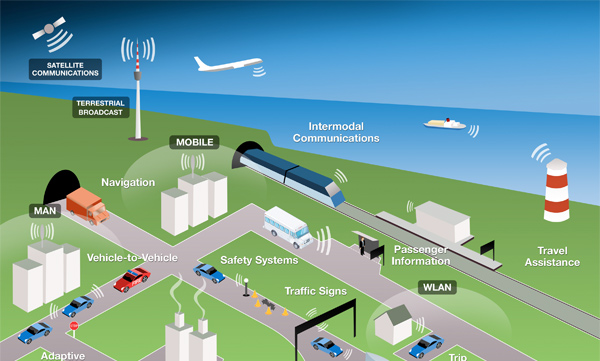
\includegraphics[width=(\textwidth)]{mass-m2m-communications.jpg}
    \caption{Model of M2M Communication network}
    \label{fig:M2M}
\end{figure}
\end{frame}
\begin{frame}{}
\begin{block}{Types of communication devices}
\begin{itemize}
    \item MTC devices (MTCD)
    \item IoT devices
\end{itemize}
\end{block}
\begin{block}{MTC}
\textbf{MTC - Machine type communication}

Machine-type communications (MTC) refer to automated data communications among devices and the underlying data transport infra-structure.
\end{block}
\begin{block}{IoT Communication}
\textbf{IoT - Internet of Things}

IoT communication protocols are modes of communication that ensure optimum security to the data being exchanged between IoT connected devices.
\end{block}
\end{frame}
\begin{frame}{MTC v/s IoT Devices}
\begin{block}{}
In some situations, providing communication services to the IoT systems is challenging due to the unavailability of a regular communication infrastructure in the deployment area.
\end{block}
\begin{block}{}
In monitoring applications, machine-type-communication devices (MTCDs) are generally deployed in areas such as deserts, forests, or even remote industrial operations, where it is hard to have access to the regular wireless communication infrastructure. In such applications, the data acquired by the MTCDs need to be timely transmitted elsewhere for further processing.
\end{block}
\end{frame}
\begin{frame}{Unfavourable terrestrial base stations}
\begin{block}{}
Deploying terrestrial wireless communication base stations is an unsatisfactory solution in situations of natural disasters or any other circumstances.
\end{block}
\begin{block}{}
Where the terrestrial base stations would have got destroyed or in a situation of cannot be used.
\end{block}
\end{frame}
\begin{frame}{}
   \LARGE{Aerial Base station(ABS) with Drones!}
   \begin{figure}[h!]
    \centering
    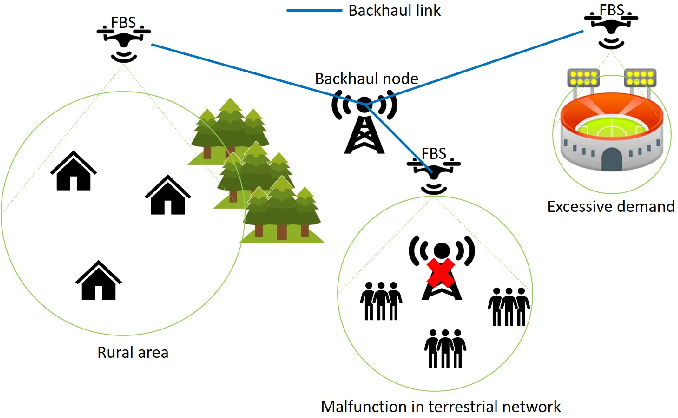
\includegraphics[width=(\textwidth)]{ABS.png}
    \caption{ABS network}
    \label{fig:ABS}
   \end{figure}
\end{frame}
\begin{frame}{Objective of this study}
    \begin{block}{}
    The main objective of this study is to devise a dynamic 3D drone placement and resource allocation technique to provide LTE coverage to an MTCD deployment in communication-congested/damaged and/or distant areas using a drone-mounted aerial base station (ABS) with near optimal radio resource scheduling under specific deployment conditions in the absence of terrestrial base stations.
    \end{block}
    \begin{block}{}
    The goal is to ensure the deployment of the drone in such a way that maximizes the communication coverage while reducing the deadline missing of the involved M2M traffic.
    \end{block}
\end{frame}
\begin{frame}{Free-space path loss model}
\begin{block}{Path loss}
 It  is the reduction in power density (attenuation) of an electromagnetic wave as it propagates through space.
\end{block}
\begin{block}{Free-space path loss}
In telecommunication, the free-space path loss (FSPL) is the attenuation of radio energy between the feed points of two antennas that results from the combination of the receiving antenna's capture area plus the obstacle-free, line-of-sight path through free space (usually air).
\end{block}
\end{frame}
\begin{frame}{}
    \begin{figure}[h!]
    \centering
    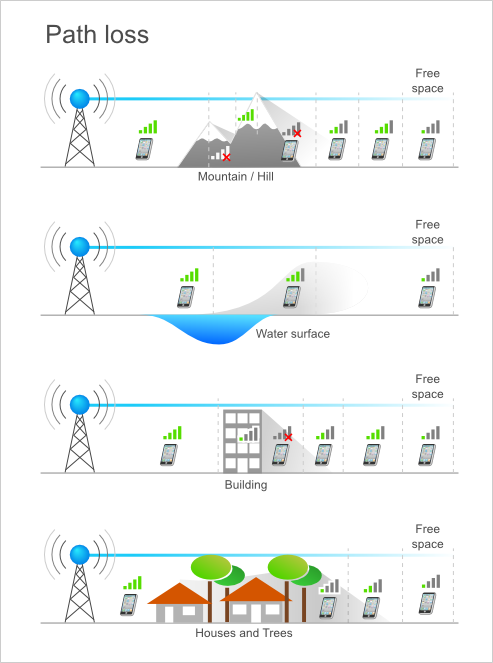
\includegraphics[width=(2.45in)]{Path_loss.png}
    \caption{Free-space Path loss}
    \label{fig:Path_loss}
   \end{figure}
\end{frame}
\begin{frame}{Path loss equation}
\begin{block}{}
The path loss equation in both line-of-sight (LoS) and non-line-of-sight (NLoS) links is given as
    \begin{align}
        L_{LoS/NLoS}=20\log\left(\frac{4\pi f_c q_i}{c}\right) + \varphi_{LoS/NLoS}
    \end{align}
\end{block}

    \begin{figure}[h!]
    \centering
    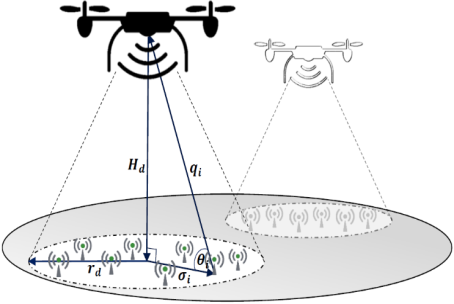
\includegraphics[width=(2.45in)]{drone.png}
    \caption{drone coverage region}
    \label{fig:drone}
   \end{figure}

\end{frame}
\begin{frame}{}
\begin{block}{}
\begin{table}[]
        \centering
\renewcommand{\arraystretch}{1.4}
        \begin{tabular}{||c|m{7cm}||}
            \hline
            Parameter & Parameter Denotes \\ 
            \hline
            \hline
            $f_c$ & carrier frequency\\ 
            \hline
            $q_i=\sqrt{H_d^2+\sigma_i^2}$ & the direct distance between an $MTCD_i$ and the drone\\ 
            \hline
            $H_d$ & the drone altitude\\ 
            \hline
            $\sigma_i$ & the ground distance between the drone perpendicular projection and an $MTCD_i$\\
            \hline
            $c$ & speed of light\\ 
            \hline
            $\varphi_{LoS/NLoS}$ & the averages of the additional losses of LoS/NLoS links respectively\\
            \hline
        \end{tabular}
        \caption{Parameters}
        \label{tab:Table1}
    \end{table}
\end{block}
\end{frame}
\begin{frame}{}
\begin{block}{Probability}
\begin{align}
    P_{NLoS}=1-P_{LoS}\\
    P_{LoS}=\frac{1}{1 + a e^{-b\left(\theta_i-a\right)}}
\end{align}
\end{block}
\begin{block}{}
\begin{table}[]
        \centering
\renewcommand{\arraystretch}{1.4}
        \begin{tabular}{||c|m{7cm}||}
            \hline
            Parameter & Parameter Denotes \\ 
            \hline
            \hline
            $P_{NLoS}$ & the probability of having NLoS links\\ 
            \hline
            $P_{LoS}$ & the probability of having LoS links\\ 
            \hline
            $a, b$ & environment-dependent factors\\
            \hline
            $\theta_i=\frac{180}{\pi}\tan^{-1}{\frac{H_d}{\sigma_i}}$ & the elevation angle\\
            \hline
        \end{tabular}
        \caption{Parameters}
        \label{tab:Table2}
    \end{table}
\end{block}
\end{frame}
\begin{frame}{}
\begin{block}{Model equation}
    The path loss equation of model is given by,
    \begin{align}
        L_{i, d} = L_{LoS}P_{LoS} + L_{NLoS}P_{NLoS}
    \end{align}
    \begin{align}
        L_{i, d} = \frac{\varphi_{LoS} - \varphi_{NLoS}}{1 + a e^{-b\left(\theta_i - a\right)}} + 10\log{\left(\sigma_{i}\sec{\theta_i}\right)} + 20\log{\left(\frac{4\pi f_{c}}{c}\right)}
    \end{align}
\end{block}
\end{frame}
\begin{frame}{Maximum permissible coverage of the drone base station}
\begin{block}{Threshold path loss}
    $\sigma_i = r_d$,
    where $r_d$ = radius of cell covered by drone
    \begin{align}
        L_{i, d}^{thr} = \frac{\varphi_{LoS} - \varphi_{NLoS}}{1 + a e^{-b\left(\theta_i - a\right)}} + 10\log{\left(r_d\sec{\theta_i}\right)} + 20\log{\left(\frac{4\pi f_{c}}{c}\right)}
    \end{align}
\end{block}
\begin{block}{Maximum achievable radius $r_d$}
    find the $\frac{\delta r_d}{\delta \theta_i}$ and equate it to $0$. We get,
    \begin{align}
        \frac{\pi}{9\ln{10}}\tan{}{\theta_i^{max}} + \frac{ab(\varphi_{LoS} - \varphi_{NLoS})e^{-b\left(\theta_i^{max} - a\right)}}{\left(1 + a e^{-b\left(\theta_i^{max} - a\right)}\right)^2} = 0
    \end{align}
    where the maximum allowable elevation angle $\theta_i^{max}$ that corresponds to the maximum achievable radius $r_d$ of the drone supported cell at $L_{i, d}^{thr}$ in conjunction with the maximum allowable height $H_d^{max}$.
\end{block}
\end{frame}
\begin{frame}{}
    \begin{block}{Data rate}
    The Data rate $R_i$ per LTE Transmission Time Interval(refers to the duration of a transmission on the radio link) is given by,
    \begin{align}
        R_i = \eta_i {BW}^{PRB}\sum\limits_{k=1}^{N_{RB}}I_{i,k}
    \end{align}
    \end{block}
    \begin{block}{}
    \begin{itemize}
        \item ${BW}^{PRB}$ is the physical resource block (PRB) bandwidth(180Hz for LTE)
        \item $\eta_i$ is spectral efficiency 
        \item $I_{i,k}$ is the a binary indicator for PRBs allocation
        \item $N_{RB}$ is the number of the available PRBs in the channel  bandwidth
    \end{itemize}
    \end{block}
    \begin{block}{PRB}
    The smallest element of resource allocated to the user.
    \end{block}
\end{frame}
\begin{frame}{}
    \begin{block}{Packet delay budget ($DB_i$)}
     The upper limit of the delay suffered by a packet.
     
    The QoS class identifier disseminates how data transmission is handled including the packet delay budget $DB_i$.
    \end{block}
    \begin{block}{}
    To calculate the total time spent on transmitting each packet, the queue model is used to estimate the distribution of the queue waiting time
    \begin{align}
        P[W_i \leq t] = \left(1 - \frac{\lambda_i}{R_i}\right)\sum\limits_{\nu = 0}^{z}\frac{\left(-\lambda_i(t - \nu T_i)\right)^\nu}{\nu!}e^{\lambda_i(t - \nu T_i)}
    \end{align}
    \end{block}
    \begin{block}{}
    \begin{itemize}
        \item $W_i$ is the waiting time of an $MTCD_i$
        \item $\lambda_i$ denotes the average arrival rate of the MTCDs’ data packets
        \item $T_i$ is the deterministic service time
        \item $z$ is an integer value such that $z T_i\leq t\leq(z+1)T_i$
    \end{itemize}
    \end{block}
\end{frame}
\begin{frame}{}
    \begin{block}{Delay time ($D_i$)}
    Total delay time of a transmission assignment can be estimated as
    \begin{align}
        D_i=W_i+T_i
    \end{align}
    \end{block}
    \begin{block}{}
    Probability of transmission deadline missing occurrence is calculated as
    \begin{align}
        P[D_i>DB_i]=1-P[D_i\leq DB_i]
    \end{align}
    \begin{align}
        P[D_i \leq DB_i] = \left(1 - \frac{\lambda_i}{R_i}\right)\sum\limits_{\nu = 0}^{z}\frac{\left(-\lambda_i(DB_i - T_i - \nu T_i)\right)^\nu}{\nu!}e^{\lambda_i(DB_i - T_i - \nu T_i)}
    \end{align}
    \end{block}
\end{frame}
\begin{frame}{}
    \begin{block}{}
    We have to maximize the number of served users and allocate the resources optimally in a way that minimizes the missed deadlines for each MTCD
    
    The optimization problem can then be written as follows,
    \begin{align}\label{eq1}
        \max\limits_{x_d, y_d, H_d, I_{i, k}}\sum\limits_{i=1}^{\mathbb{U}} u_i
    \end{align}
    \begin{align}
        H_d^{min} \leq H_d \leq H_d^{max}\\
        P[D_i > DB_i] \leq {DM}_i^{max}, \forall i \in u_s\\
        \sum\limits_{i=0}^{u_s}I_{i,k}\leq 1, \forall k \in N_{RB}\\
        x_d, y_d, H_d \in \mathbb{R}\\
        u_i\in\{0,1\}, I_{i,k}\in\{0,1\}, \forall i\in \mathbb{U}, k \in N_{RB}
    \end{align}
    \end{block}
\end{frame}
\begin{frame}{}
    \begin{block}{}
    \begin{itemize}
        \item $u_i$ is a binary index to indicate the geographically location of an $MTCD_i$
        \begin{align}
            u_i =
            \begin{cases}
                    1, & \sigma_i\leq r_d\\
                    0, & \sigma_i>r_d
            \end{cases}
        \end{align}
        \item $u_s$ is the subset representing the active MTCDs of the set $\mathbb{U}$ of the total deployed MTCDs
        \item $x_d$ and $y_d$ are the ABS’s 2D location
        \item $H_d^{min}$ is lower bound of the drone’s altitude
        \item $DM_i^{max}$ is the allowable probability of missing a deadline coordinates
        \item $\sigma_i=\sqrt{(x_i-x_d)^2+(y_i-y_d)^2}$
        \item $r_d=H_d\cot{\theta_i^{max}}$, where $r_d$ is radius of disk shaped coverage area of ABS
    \end{itemize}
    \end{block}
\end{frame}
\begin{frame}{}
    \begin{block}{Penalty method}
    A penalty method replaces a constrained optimization problem by a series of unconstrained problems whose solutions ideally converge to the solution of the original constrained problem
    \end{block}
    \begin{block}{}
    The derived objective function is solved by one of the unconstrained conventional meta-heuristic methods.
    
    The problem in \eqref{eq1} is reformulated as
    \begin{multline}\label{eq2}
        \max\limits_{x_d, y_d, H_d, I_{i, k}} f(x_d, y_d, H_d, I_{i, k}) = \sum\limits_{i = 1}^{\mathbb{U}}u_i -\\ \sum\limits_{i = 1}^{u_s}\psi_i\max(0,P[D_i > DB_i] - DM_i^{max})^2, \psi_i>0
    \end{multline}
    \end{block}
    \begin{block}{}
    \begin{itemize}
        \item  $f(x_d, y_d, H_d, I_{i, k})$ is the unconstrained objective function
        \item $\psi_i$ is the penalty coefficient
    \end{itemize}
\end{block}
\end{frame}
\begin{frame}{}
\begin{block}{Particle swarm optimization(PSO)}
It is a computational method that optimizes a problem by iteratively trying to improve a candidate solution concerning a given measure of quality.
\end{block}
\begin{block}{}
We solve \eqref{eq2} using the PSO algorithm. The algorithm updates each particle’s position $P_s$ that represents a row vector including the 3D drone placement and the PRBs scheduling scheme. This is done by updating its associated direction and speed $V_{s,n}$.
\begin{align}
    V_{s,n}=w V_{s,n}+c_1r_1(Pb_{s,n}-P_{s,n})+c_2r_2(Gb_{n}-P_{s,n})
\end{align}
\end{block}
\begin{block}{}
\begin{itemize}
    \item $c_1$ and $c_2$ are the acceleration constants
    \item $r_1$ and $r_2$ are uniformly distributed random variables
    \item $w$ is the inertia weight constant
    \item $Gb_n$ and $Pb_{s,n}$ are the global and personal best positions
\end{itemize}
\end{block}
\end{frame}
\begin{frame}{}
    \begin{block}{}
    \begin{itemize}
        \item The probability of changing a binary state is introduced to reformulate the velocity concept in the generic PSO.
        \item This algorithmic solution integrates the unified model of PSO to allow the particles to learn from not only the personal and the global exemplars but the local exemplar as well to provide wide exploration to the search space
    \end{itemize}
    The particles’ velocities are updated as
    \begin{align}
        V_{s,n}=\alpha\times GV_n + r(1 - \alpha)LV_{s,n}
    \end{align}
    \end{block}
    \begin{block}{}
    \begin{itemize}
        \item $\alpha$ is a unification factor
        \item $r$ is a normally distributed random number
        \item $GV_n$ and $LV_{s,n}$ are velocities of global and local exemplars
    \end{itemize}
    \end{block}
    \begin{block}{}
        A ring topology of size $rg$ is used to specify the local neighbors of each particle.
    \end{block}
\end{frame}
\begin{frame}{}
    \begin{figure}[h!]
    \centering
    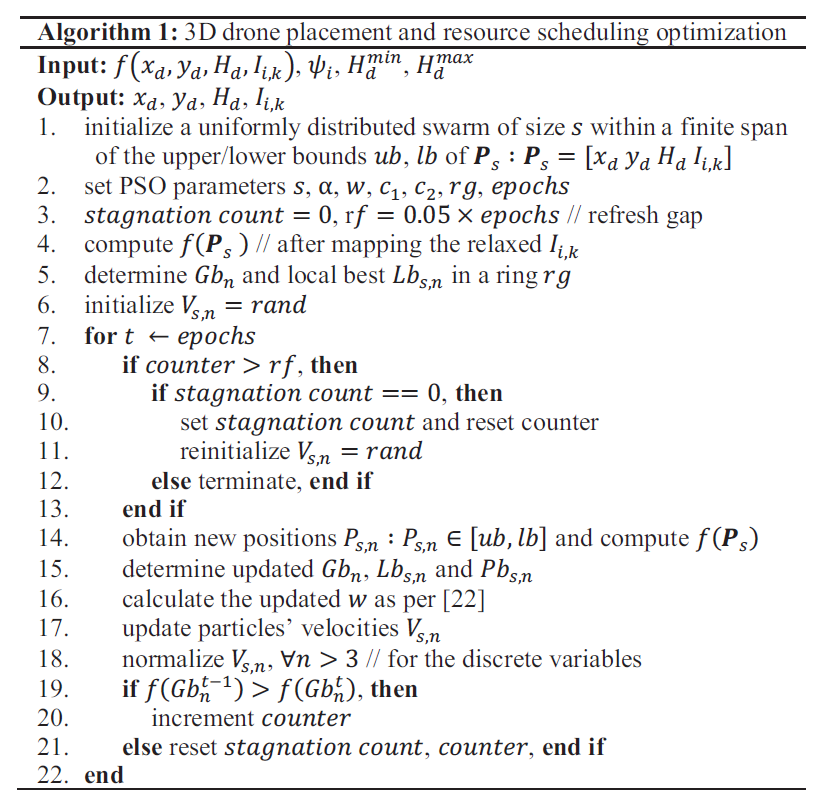
\includegraphics[width=(9.4cm)]{Algorithm.png}
    \label{fig:Algorithm}
    \end{figure}
\end{frame}
\title{Simulation}
\author{}
\begin{frame}{}
    \titlepage
\end{frame}
\begin{frame}{}
    \begin{block}{}
    \begin{table}[]
        \centering
        \renewcommand{\arraystretch}{1.4}
        \begin{tabular}{||c|m{4cm}||}
            \hline
            Parameter & Value \\ 
            \hline
            \hline
            Channel Bandwidth, Carrier Frequency $f_c$ & 3 MHz, 2 GHz\\ 
            \hline
            Number of PRBs and LTE Frames & 15, 100\\ 
            \hline
            Number of Deployed MTCDs & 100, 150, 200, 250, 300\\
            \hline
            Deployed MTCDs’ Density & 11 $MTCDs/km^2$\\
            \hline
            Environment Parameters a, b, $\varphi_{LoS}$, $\varphi_{NLoS}$ & 5.0188, 0.3511, 0.1, 21\\
            \hline
            Transmission and Noise Power & 30, -70 dBm\\
            \hline
            Deadline Missing Probability $DM_i^{max}$ & $10\%$\\
            \hline
            PSO Parameters $s$, $\alpha$, $w$, $c_1$, $c_2$ & 50, 0.1, 0.729, 1.494, 1.494\\
            \hline
            $rg$, $epochs$ & 5, 250\\
            \hline
        \end{tabular}
        \label{tab:Table3}
    \end{table}
    \end{block}
\end{frame}
\begin{frame}{}
    \begin{block}{}
    \begin{table}[]
        \centering
        \renewcommand{\arraystretch}{1.4}
        \begin{tabular}{||c|c|c|m{2cm}||}
            \hline
            Traffic Description & Alerts & Camera & Monitoring Sensor \\ 
            \hline
            \hline
            Arrival Rate (pkt/s) & 25 & 30 & 1\\ 
            \hline
            Packet Size (byte) & 32 & 512 & 128\\ 
            \hline
            Profile Percentage\% & 20 & 20 & 60\\
            \hline
            Threshold Path Loss (dB) & 95 & 98 & 100\\
            \hline
            Delay Budget (ms) & U(10,20) & U(125,250) & U(800,900)\\
            \hline
        \end{tabular}
        \label{tab:Table3}
    \end{table}
    \end{block}
\end{frame}
\begin{frame}{Overall system deadline missing ratio}
    \begin{figure}[h!]
    \centering
    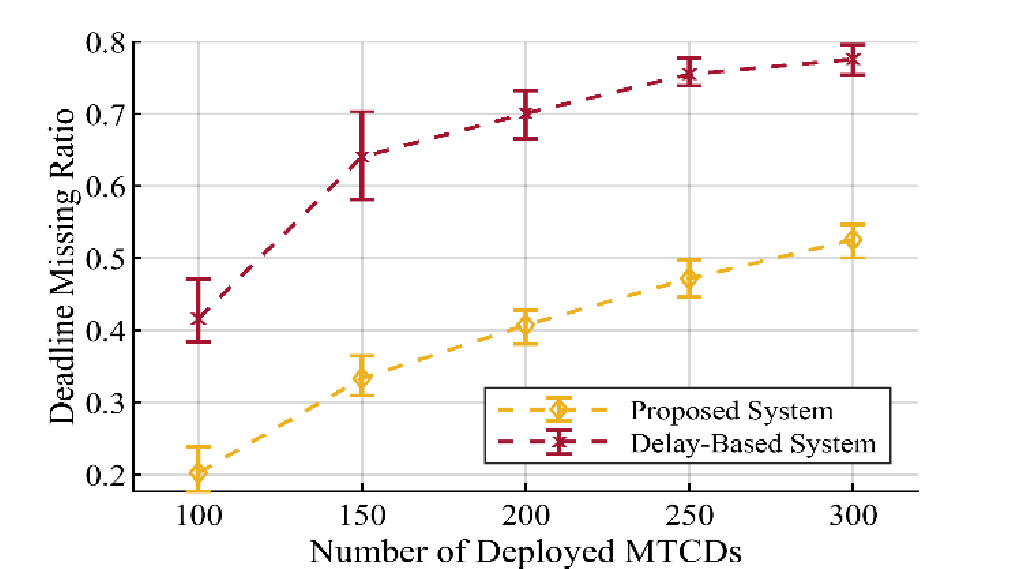
\includegraphics[width=(11cm)]{Overall system deadline missing ratio.png}
    \label{fig:overalldeadline}
    \end{figure}
\end{frame}
\begin{frame}{System agregate througput}
    \begin{figure}[h!]
    \centering
    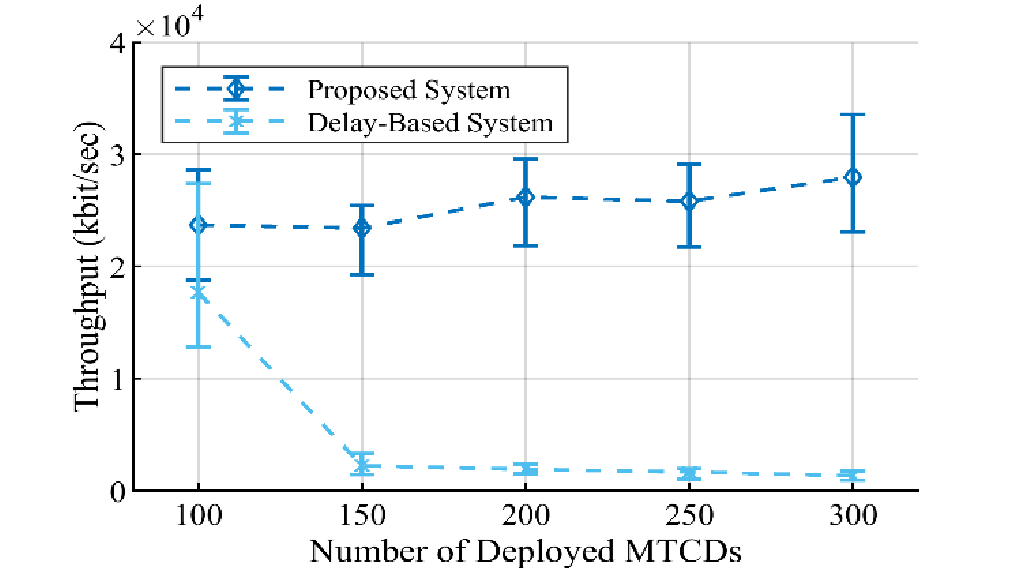
\includegraphics[width=(11cm)]{System agregate througput.png}
    \label{fig:systemthroughput}
    \end{figure}
\end{frame}
\begin{frame}{Alarms deadline missing ratio}
    \begin{figure}[h!]
    \centering
    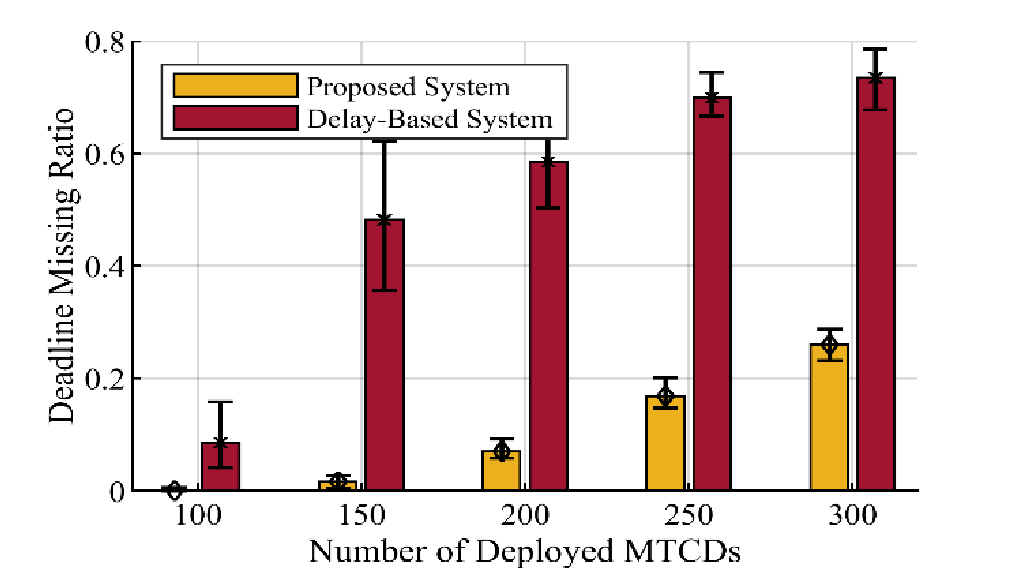
\includegraphics[width=(11cm)]{Alarms deadline missing ratio.png}
    \label{fig:systemthroughput}
    \end{figure}
\end{frame}
\begin{frame}{Camera traffic throughput}
    \begin{figure}[h!]
    \centering
    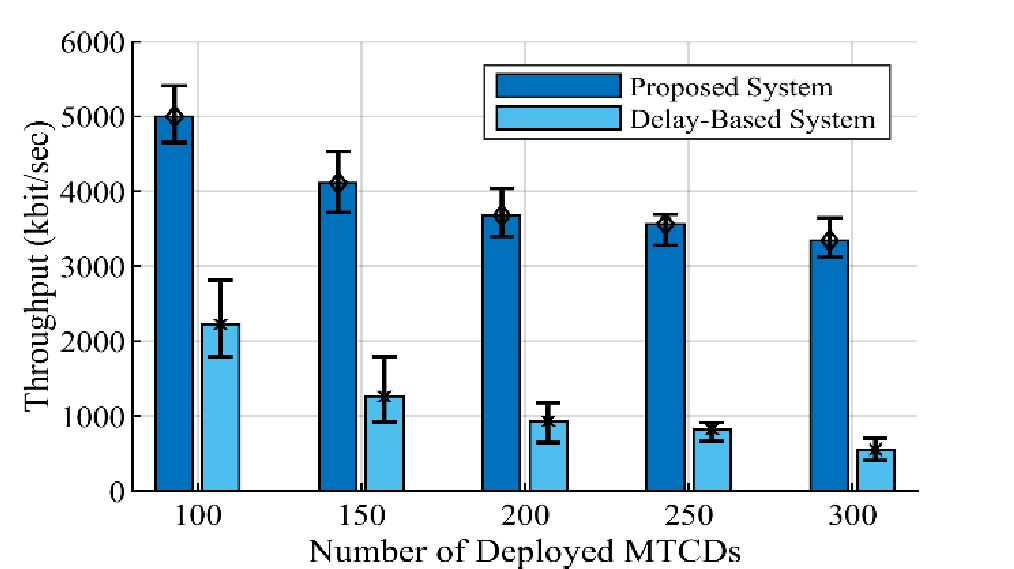
\includegraphics[width=(11cm)]{Camera traffic throughput.png}
    \label{fig:systemthroughput}
    \end{figure}
\end{frame}
\begin{frame}{Number of Deployed MTCDs}
    \begin{figure}[h!]
    \centering
    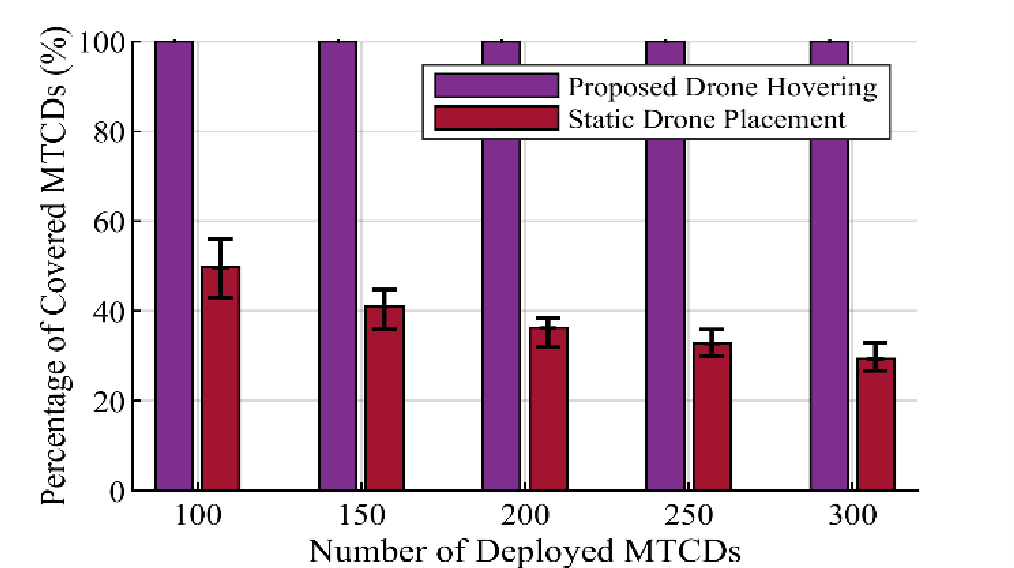
\includegraphics[width=(11cm)]{Number of Deployed MTCDs.png}
    \label{fig:systemthroughput}
    \end{figure}
\end{frame}

\end{document}